Ripeto la regressione polinomiale dell'esercizio precedente con l'aggiunta di regolarizzatore (bias).

Con l'uso del $ bias $ $\lambda$ cerco di regolarizzare il mio polinomio: in sostanza aumetando lambda semplifico il mio risultato mentre dimunendolo utilizzo una funzione più complessa per la regressione, quindi modificare $\lambda$ è concettualmente simile a cambiare il grado del polinomio, offrendo, però, una maggior granularità nella scelta del valore ottimale.
$\lambda$ rappresenta il livello di fiducia nella qualità dei dati in ingresso: più l'ingresso è rumoroso più conviene utilizzare $\lambda$ grandi e quindi adottare soluzioni semplici in modo to not fit the noise, meno è rumoroso e più possiamo diminuire $\lambda$ ed utilizzare soluzioni più comlplesse in order to fit data.

In this exercise it's repeated the polynomial regression of the previous one with the addition of a regularizer $bias$.
With the use of $ bias $ $\lambda$ we try to regularize our polynomial: so by stretching $\lambda$ we simplify my result while using it to use a more complex function for regression, so modifying $\lambda$ is conceptually similar to changing the degree of polynomial, offering, however, a greater granularity in the choice of the optimal value.
$\lambda$ represents the level of confidence in the quality of input data: the more noisy the input, the better it's to use $\lambda$ large and then adopt simple solutions to not fit the noise, the less it is noisy and the more we can decrease $\lambda$ and use more complex solutions in order to fit data.

\begin{figure}[h]
	\centering
	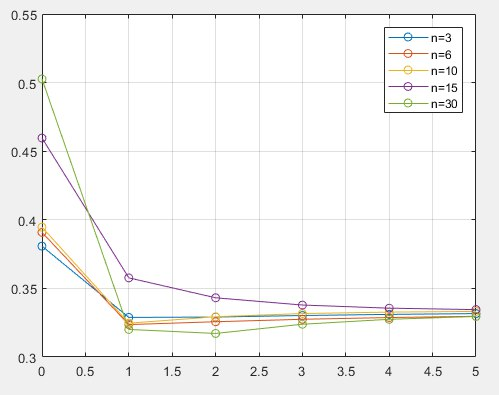
\includegraphics[width=0.5\textwidth]{pl100s10.png}
\end{figure}

\begin{figure}[h]
	\centering
	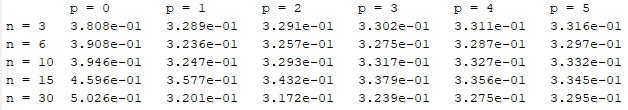
\includegraphics[width=0.5\textwidth]{tl100s10.png}
	\caption{$\lambda$ = 100 $\sigma$ = 10}
	\label{fig:lambda = 100 sigma = 10}
\end{figure}

\begin{figure}[h]
	\centering
	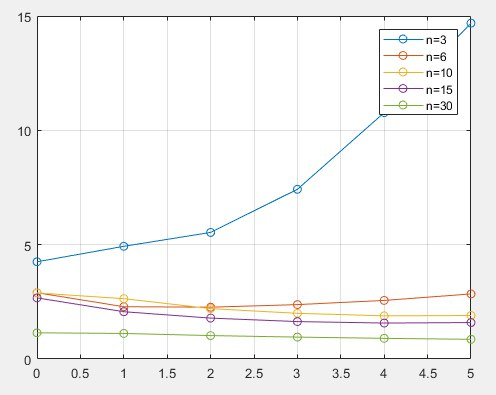
\includegraphics[width=0.5\textwidth]{pl0001s10.png}
\end{figure}

\begin{figure}[h]
	\centering
	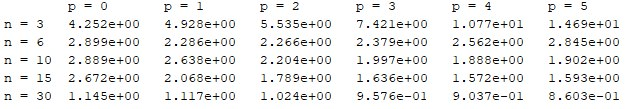
\includegraphics[width=0.5\textwidth]{tl0001s10.png}
	\caption{$\lambda$ = 0,001 $\sigma$ = 10}
	\label{fig:lambda = 0,001 sigma = 10}
\end{figure}

\begin{figure}[h]
	\centering
	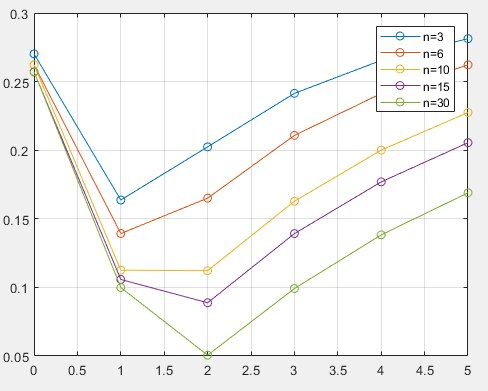
\includegraphics[width=0.5\textwidth]{pl1s001.png}
\end{figure}

\begin{figure}[h]
	\centering
	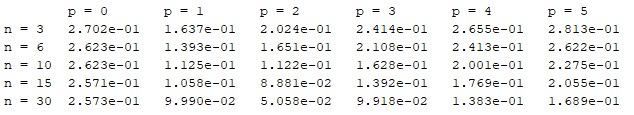
\includegraphics[width=0.5\textwidth]{tl1s001.png}
	\caption{$\lambda$ = 1 $\sigma$ = 0,01}
	\label{fig:lambda = 1 sigma = 0,01}
\end{figure}

\begin{figure}[h]
	\centering
	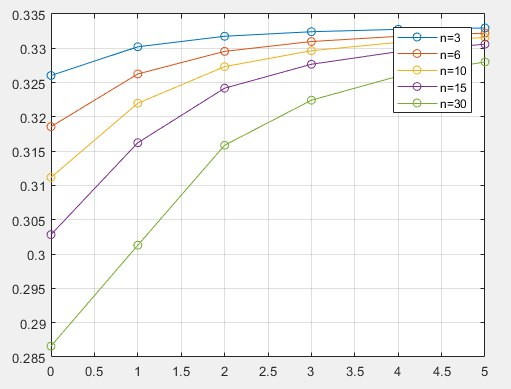
\includegraphics[width=0.5\textwidth]{pl100s01.png}
\end{figure}

\begin{figure}[h]
	\centering
	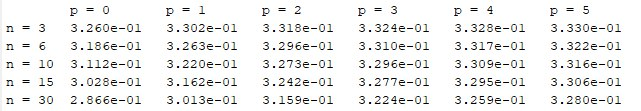
\includegraphics[width=0.5\textwidth]{tl100s01.png}
	\caption{$\lambda$ = 100 $\sigma$ = 0,01}
	\label{fig:lambda = 100 sigma = 0,01}
\end{figure}

\begin{figure}[h]
	\centering
	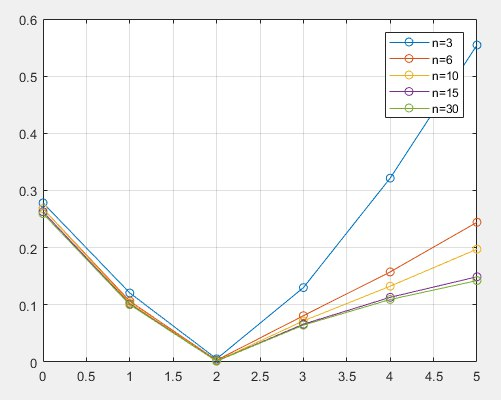
\includegraphics[width=0.5\textwidth]{pl000001s001.png}
\end{figure}

\begin{figure}[h]
	\centering
	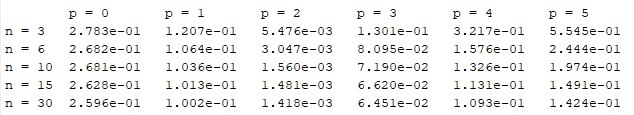
\includegraphics[width=0.5\textwidth]{tl000001s001.png}
	\caption{$\lambda$ = 0,00001 $\sigma$ = 0,01}
	\label{fig:lambda = 0,00001 sigma = 0,01}
\end{figure}